\documentclass[12pt]{article}
\usepackage[utf8]{inputenc}
\usepackage[brazilian]{babel}
\usepackage{geometry}
\geometry{a4paper, total={170mm,250mm}, left=25mm, right=25mm, top=25mm}
\usepackage{graphicx}
\usepackage{titling}
\usepackage{float}
\usepackage{amsmath}

\title{Lista de Exercícios 2 - MEC2403 (Otimização)}
\author{Kleyton da Costa (2312730)}
\date{\today}
 
\usepackage{fancyhdr}
\fancypagestyle{plain}{%  the preset of fancyhdr 
    \fancyhf{} % clear all header and footer fields
    %\fancyfoot[R]{\includegraphics[width=3cm]{di.png}}
    \fancyfoot[L]{\today}
    \fancyhead[L]{Lista de Exercícios}
    \fancyhead[R]{\theauthor}
}
\makeatletter
\def\@maketitle{%
  \newpage
  \null
  \vskip 1em%
  \begin{center}%
  \let \footnote \thanks
    {\LARGE \@title \par}%
    \vskip 1em%
    %{\large \@date}%
  \end{center}%
  \par
  \vskip 1em}
\makeatother

\begin{document}

\maketitle

\noindent\begin{tabular}{@{}ll}
    Aluno & \theauthor \\
    Professor &  Ivan Menezes (MEC/PUC-Rio) \\
    Data & \today
\end{tabular}

\section*{Exercício 2}

\subsection*{Letra (a)}

\begin{equation}
f(x_{1}, x_{2})= x_{1}^{2}-3x_{1}x_{2}+4x_{2}^{2}+x_{1}-x_{2}
\end{equation}

\begin{itemize}
    \item Ponto inicial: $x^{0}=\{1,2\}^{t}$
    \item Direção: $d = \{-1, -2\}^{t}$ 
\end{itemize}

\begin{figure}[H]
    \centering
    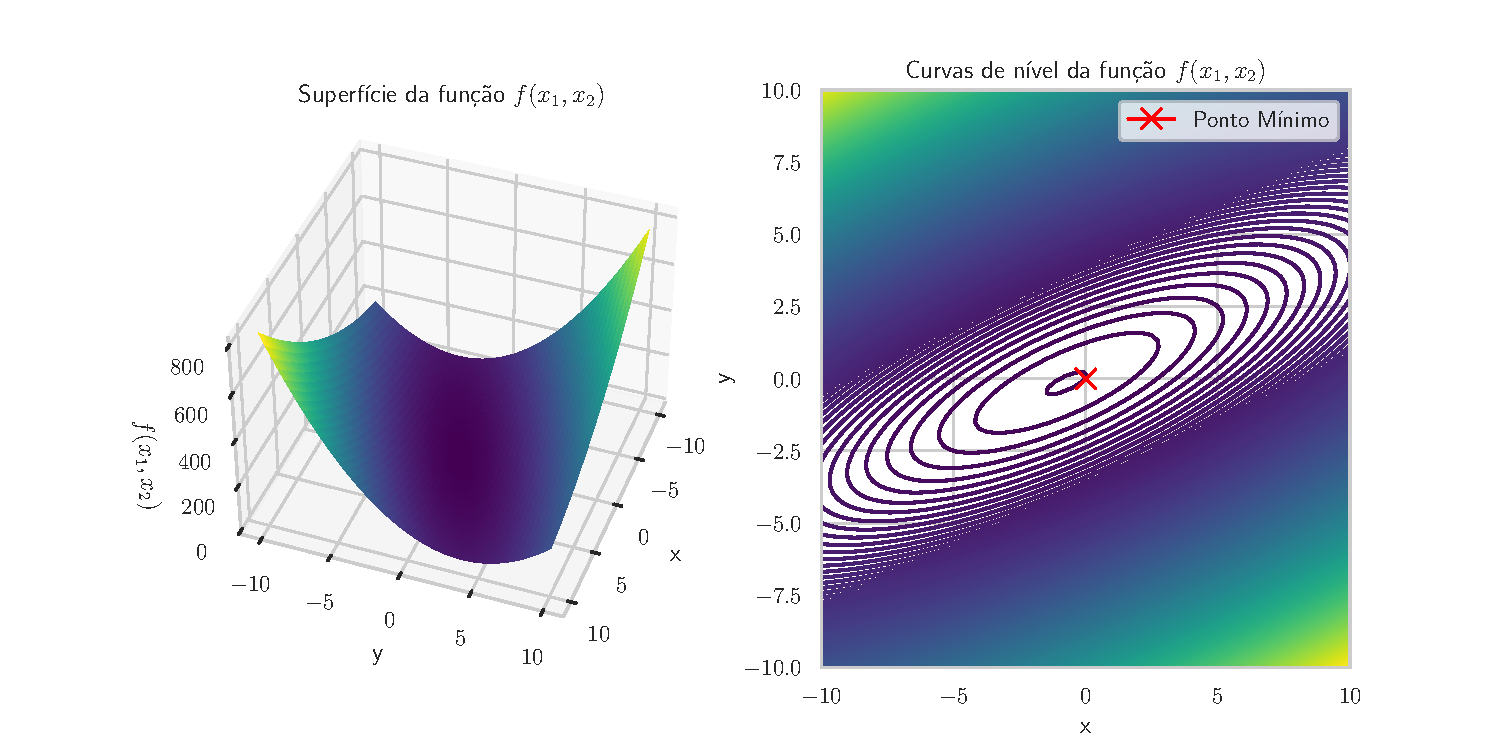
\includegraphics[scale = 0.6]{figures/questao_2a.pdf}
    \caption{Minização através da seção áurea}
\end{figure}


\subsection*{Letra (b)}

\paragraph{Função de MacCormick}

\begin{equation}
    f(x_{1}, x_{2}) = sin(x_{1}+x_{2}) + (x_{1}-x_{2})^{2}-1.5x_{1}+2.5x_{2}
\end{equation}

\begin{itemize}
    \item Ponto inicial: $x^{0} = \{-2,3\}^{t}$
    \item Direção: $d = \{1.453, -4.547\}^{t}$
\end{itemize}

\begin{figure}[H]
    \centering
    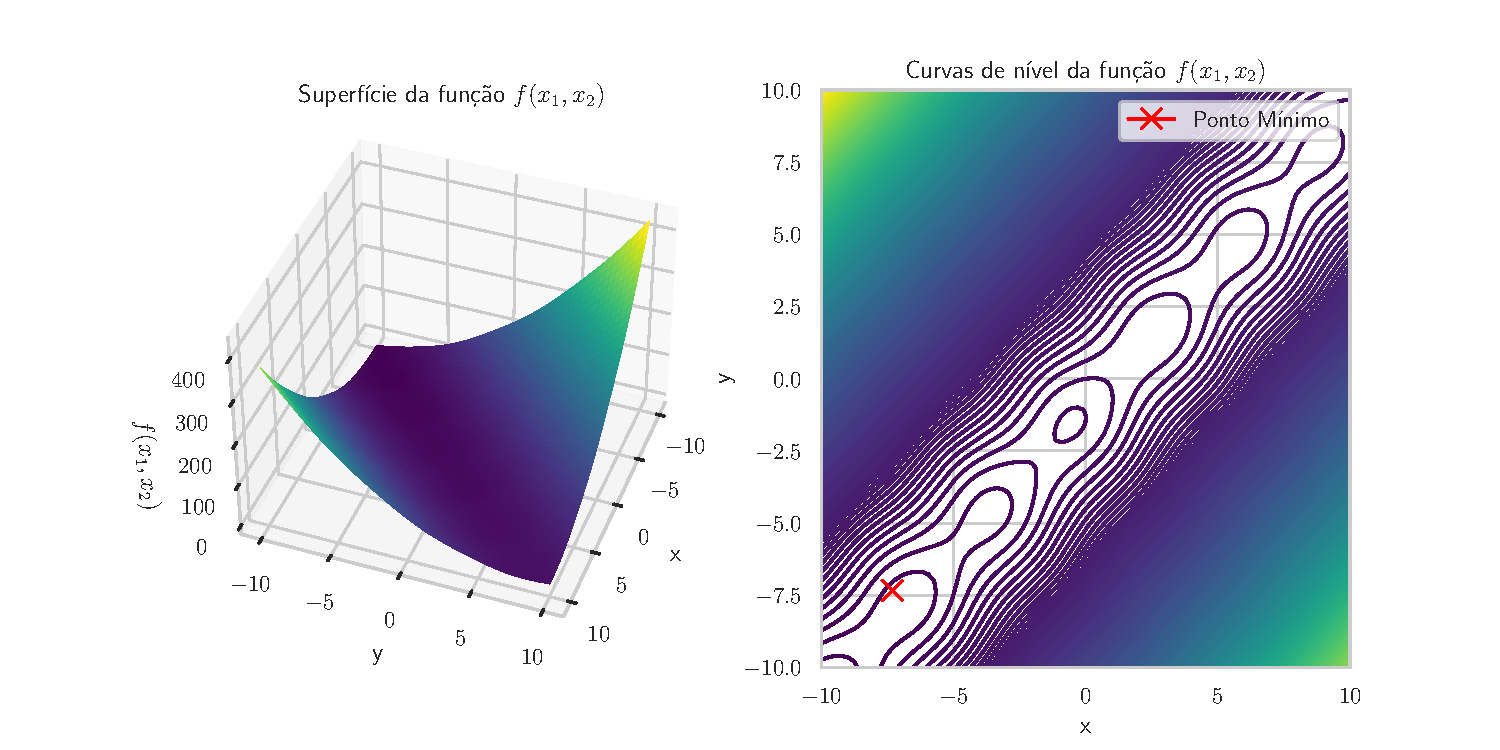
\includegraphics[scale = 0.6]{figures/questao_2b.pdf}
    \caption{Minização através da seção áurea}
\end{figure}

\subsection{Letra (c)}

\paragraph{Função de Himmelblau}

\begin{equation}
(c) ~~ f(x_{1}, x_{2}) = (x_{1}^{2}+x_{2}-11)^{2} + (x_{1}+x_{2}^{2}-7)^{2}
\end{equation}

\begin{itemize}
    \item Ponto inicial: $x^{0}=\{0,5\}^{t}$
    \item Direção: $d=\{3,1.5\}^{t}$
\end{itemize}

\begin{figure}[H]
    \centering
    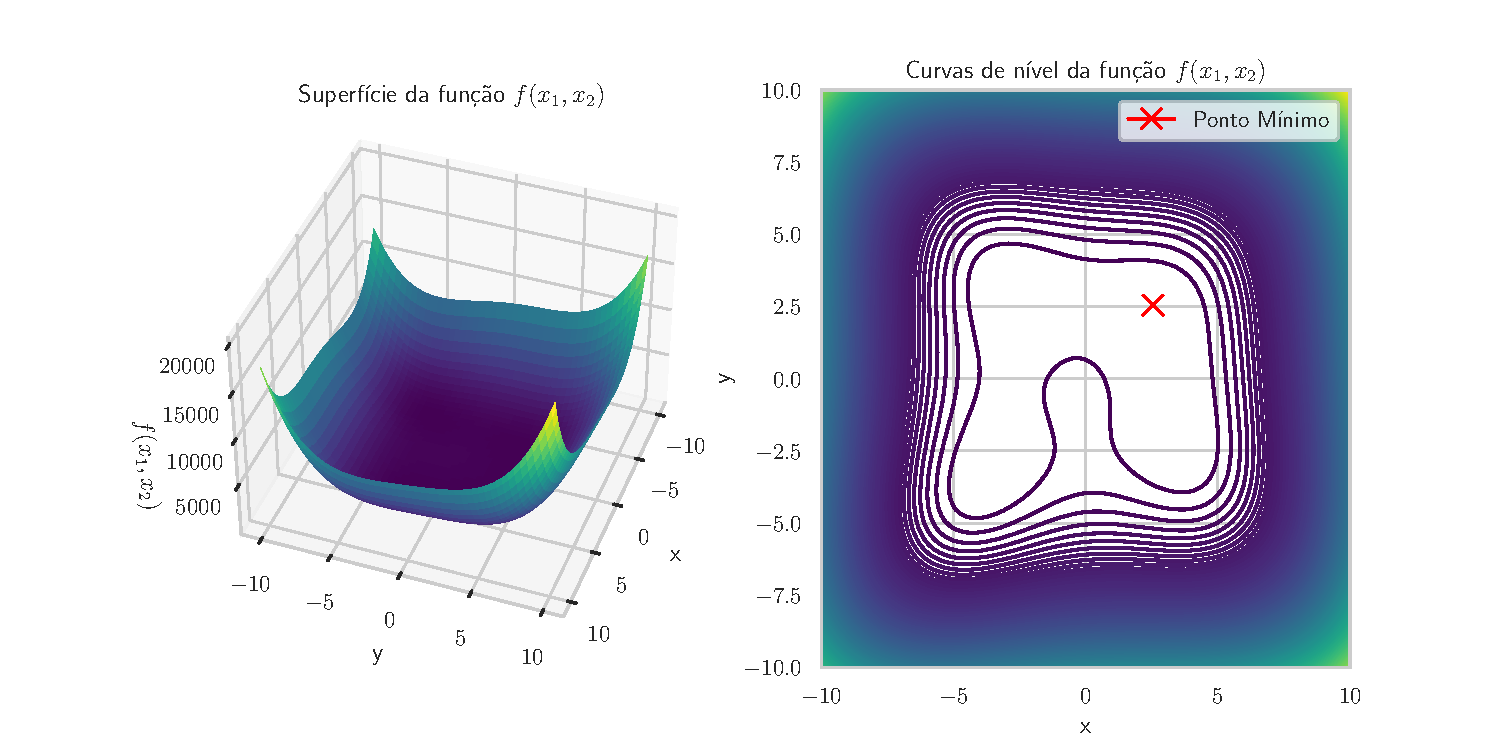
\includegraphics[scale = 0.6]{figures/questao_2c.pdf}
    \caption{Minização através da seção áurea}
\end{figure}


\end{document}
